\documentclass[a4paper,12pt]{article}

\usepackage[utf8]{inputenc}
\usepackage{amsmath,amssymb,amsfonts}
\usepackage{graphicx}
\usepackage{hyperref}
\usepackage{physics}
\usepackage{float}
\usepackage{caption}
\usepackage{subcaption}
\usepackage{geometry}
\geometry{margin=2.5cm}

\title{Studio del Problema degli \textit{n}-corpi gravitazionali in 3D: studio analitico, confronto tra metodi numerici e studio della caoticità}
\author{Carlo Lodin, Giacomo Fundarò}
\date{07/04/2025}

\begin{document}

\maketitle

\section{Introduzione}
Il problema degli \textit{n}-corpi consiste nello studio del moto di $n$ masse puntiformi che interagiscono tra loro per mezzo della forza gravitazionale. Si tratta di un problema classico della meccanica celeste, non risolvibile in forma chiusa per $n > 2$, il che rende necessaria un'approssimazione numerica per l'analisi del sistema. In questo lavoro si simula il sistema in 3D e si confrontano quattro metodi numerici: Eulero esplicito, Eulero simplettico, Verlet e Runge-Kutta del quarto ordine.


\section{Studio lagrangiano del sistema}

Consideriamo un sistema di \( n \) corpi puntiformi con masse \( m_1, \dots, m_n \), soggetti all'interazione gravitazionale newtoniana. La posizione del corpo \( i \)-esimo è descritta da \( \mathbf{r}_i(t) \in \mathbb{R}^3 \), e la sua velocità da \( \dot{\mathbf{r}}_i(t) \).

\subsection{Lagrangiana del sistema}

La lagrangiana \( \mathcal{L} \) è definita come differenza tra energia cinetica totale e energia potenziale gravitazionale:

\[
\mathcal{L}(\mathbf{r}_1, \dots, \mathbf{r}_n, \dot{\mathbf{r}}_1, \dots, \dot{\mathbf{r}}_n) = 
\sum_{i=1}^n \frac{1}{2} m_i \|\dot{\mathbf{r}}_i\|^2 + 
\sum_{1 \leq i < j \leq n} \frac{G m_i m_j}{\|\mathbf{r}_i - \mathbf{r}_j\|}
\]

dove \( G \) è la costante gravitazionale.

\subsection{Equazioni di Eulero-Lagrange}

Le equazioni del moto si ottengono applicando le equazioni di Eulero-Lagrange a ciascun corpo:

\[
\frac{d}{dt} \left( \frac{\partial \mathcal{L}}{\partial \dot{\mathbf{r}}_i} \right) - \frac{\partial \mathcal{L}}{\partial \mathbf{r}_i} = \mathbf{0}
\]

\paragraph{Primo termine: derivata rispetto alla velocità}

\[
\frac{\partial \mathcal{L}}{\partial \dot{\mathbf{r}}_i} = \frac{\partial}{\partial \dot{\mathbf{r}}_i} \left( \sum_{k=1}^n \frac{1}{2} m_k \|\dot{\mathbf{r}}_k\|^2 \right) = m_i \dot{\mathbf{r}}_i
\]

quindi:

\[
\frac{d}{dt} \left( \frac{\partial \mathcal{L}}{\partial \dot{\mathbf{r}}_i} \right) = m_i \ddot{\mathbf{r}}_i
\]

\paragraph{Secondo termine: derivata rispetto alla posizione}

Solo il termine potenziale dipende dalle posizioni \( \mathbf{r}_i \). La derivata parziale è:

\[
\frac{\partial \mathcal{L}}{\partial \mathbf{r}_i} = \frac{\partial}{\partial \mathbf{r}_i} \left( \sum_{1 \leq k < l \leq n} \frac{G m_k m_l}{\|\mathbf{r}_k - \mathbf{r}_l\|} \right)
\]

Il termine che contiene \( \mathbf{r}_i \) è quello in cui \( i = k \) o \( i = l \). Per ciascuna coppia \( (i, j) \), otteniamo:

\[
\frac{\partial}{\partial \mathbf{r}_i} \left( \frac{1}{\|\mathbf{r}_i - \mathbf{r}_j\|} \right) = \frac{\mathbf{r}_i - \mathbf{r}_j}{\|\mathbf{r}_i - \mathbf{r}_j\|^3}
\]

quindi:

\[
\frac{\partial \mathcal{L}}{\partial \mathbf{r}_i} = -G \sum_{\substack{j=1 \\ j \ne i}}^n m_i m_j \frac{\mathbf{r}_i - \mathbf{r}_j}{\|\mathbf{r}_i - \mathbf{r}_j\|^3}
\]

\paragraph{Equazioni del moto}

Sostituendo nella legge di Eulero-Lagrange:

\[
m_i \ddot{\mathbf{r}}_i = -\frac{\partial \mathcal{L}}{\partial \mathbf{r}_i} = G \sum_{\substack{j=1 \\ j \ne i}}^n m_i m_j \frac{\mathbf{r}_j - \mathbf{r}_i}{\|\mathbf{r}_i - \mathbf{r}_j\|^3}
\]

Dividendo per \( m_i \), si ottiene la forma finale:

\[
\ddot{\mathbf{r}}_i = G \sum_{\substack{j=1 \\ j \ne i}}^n m_j \frac{\mathbf{r}_j - \mathbf{r}_i}{\|\mathbf{r}_i - \mathbf{r}_j\|^3}
\]

che rappresenta l'accelerazione del corpo \( i \) per effetto dell'interazione gravitazionale con tutti gli altri corpi del sistema.

\section{Studio hamiltoniano del sistema}
Il formalismo hamiltoniano introduce le coordinate generalizzate $\vb{r}_i$ e i momenti coniugati $\vb{p}_i = m_i \dot{\vb{r}}_i$. L'hamiltoniana \`e data dall'energia totale del sistema:
\begin{equation}
    \mathcal{H} = T + V = \sum_{i=1}^n \frac{\vb{p}_i^2}{2m_i} - \sum_{i<j} \frac{G m_i m_j}{\norm{\vb{r}_i - \vb{r}_j}}
\end{equation}

Le equazioni di Hamilton sono:
\begin{equation}
\begin{cases}
    \dot{\vb{r}}_i = \pdv{\mathcal{H}}{\vb{p}_i} = \frac{\vb{p}_i}{m_i} \\
    \dot{\vb{p}}_i = -\pdv{\mathcal{H}}{\vb{r}_i} = -G m_i \sum_{j \neq i} m_j \frac{\vb{r}_i - \vb{r}_j}{\norm{\vb{r}_i - \vb{r}_j}^3}
\end{cases}
\end{equation}
Da cui si giunge alle stesse equazioni ottenute nella sezione 2. Pertanto, le stesse formule possono essere utilizzate con integratori simplettici.

\section{Implementazione numerica}
Il sistema \`e stato simulato in MATLAB. \\I corpi vengono inizializzati con una distribuzione tridimensionale, con un corpo centrale e gli altri disposti attorno ad esso con velocit\`a iniziali tangenziali. Sono stati implementati i seguenti metodi numerici:

\subsection*{Eulero esplicito}
Aggiorna prima la posizione, poi la velocit\`a:
\begin{equation}
    \vb{r}_i^{t+\Delta t} = \vb{r}_i^t + \Delta t \vb{v}_i^t
\end{equation}
\begin{equation}
    \vb{v}_i^{t+\Delta t} = \vb{v}_i^t + \Delta t \vb{a}_i^t
\end{equation}
Tale metodo ha il vantaggio di essere molto semplice, tuttavia è spesso instabile.

\subsection*{Eulero simplettico}
Aggiorna prima la velocit\`a, poi la posizione:
\begin{equation}
    \vb{v}_i^{t+\Delta t} = \vb{v}_i^t + \Delta t \vb{a}_i^t
\end{equation}
\begin{equation}
    \vb{r}_i^{t+\Delta t} = \vb{r}_i^t + \Delta t \vb{v}_i^{t+\Delta t}
\end{equation}
Conserva meglio l'energia rispetto a Eulero esplicito.

\subsection*{Velocity Verlet}
Metodo simplettico con ottime proprietà di stabilità e precisione:
\begin{align}
    \vb{r}_i^{t+\Delta t} &= \vb{r}_i^t + \vb{v}_i^t \Delta t + \frac{1}{2} \vb{a}_i^t \Delta t^2 \\
    \vb{a}_i^{t+\Delta t} &= f(\vb{r}^{t+\Delta t}) \\
    \vb{v}_i^{t+\Delta t} &= \vb{v}_i^t + \frac{\vb{a}_i^t + \vb{a}_i^{t+\Delta t}}{2} \Delta t
\end{align}

\subsection*{Runge-Kutta 4}
Metodo ad alta precisione, non simplettico:
\begin{equation}
    \vb{y}_{t+\Delta t} = \vb{y}_t + \frac{\Delta t}{6}(k_1 + 2k_2 + 2k_3 + k_4)
\end{equation}
con $k_i$ che stimano la pendenza alle diverse frazioni del passo.

\section{Comparazione dei metodi}
Sono stati eseguiti esperimenti con i quattro metodi a parit\`a di condizioni iniziali con dt=0.01. Sono stati monitorati: l'energia totale e le traiettorie dei corpi. \\Riportiamo di seguito un esempio di simulazione mettendo a confronto i quattro metodi.

\begin{figure}[H]
    \centering
    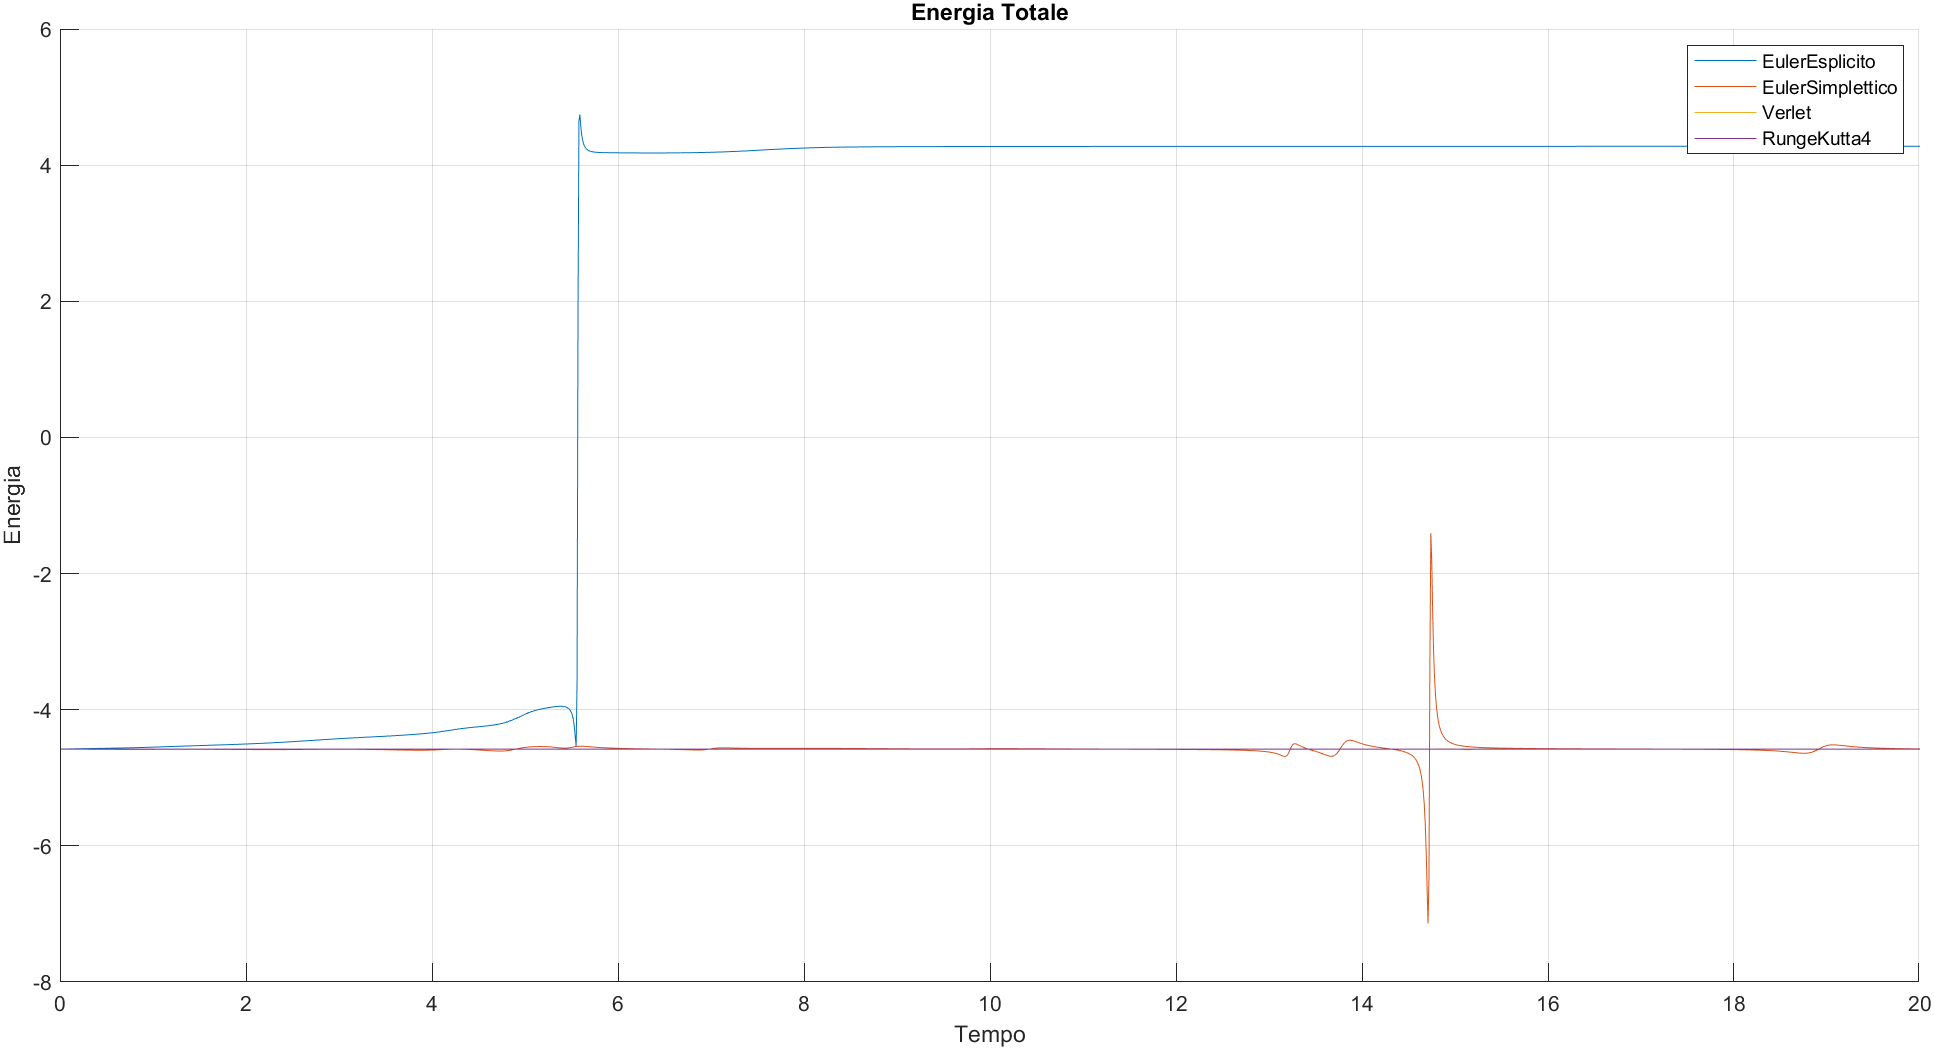
\includegraphics[width=1\textwidth]{energy_plot.png}
    \caption{Energia totale del sistema per ogni metodo.}
\end{figure}

\begin{figure}[H]
    \centering
    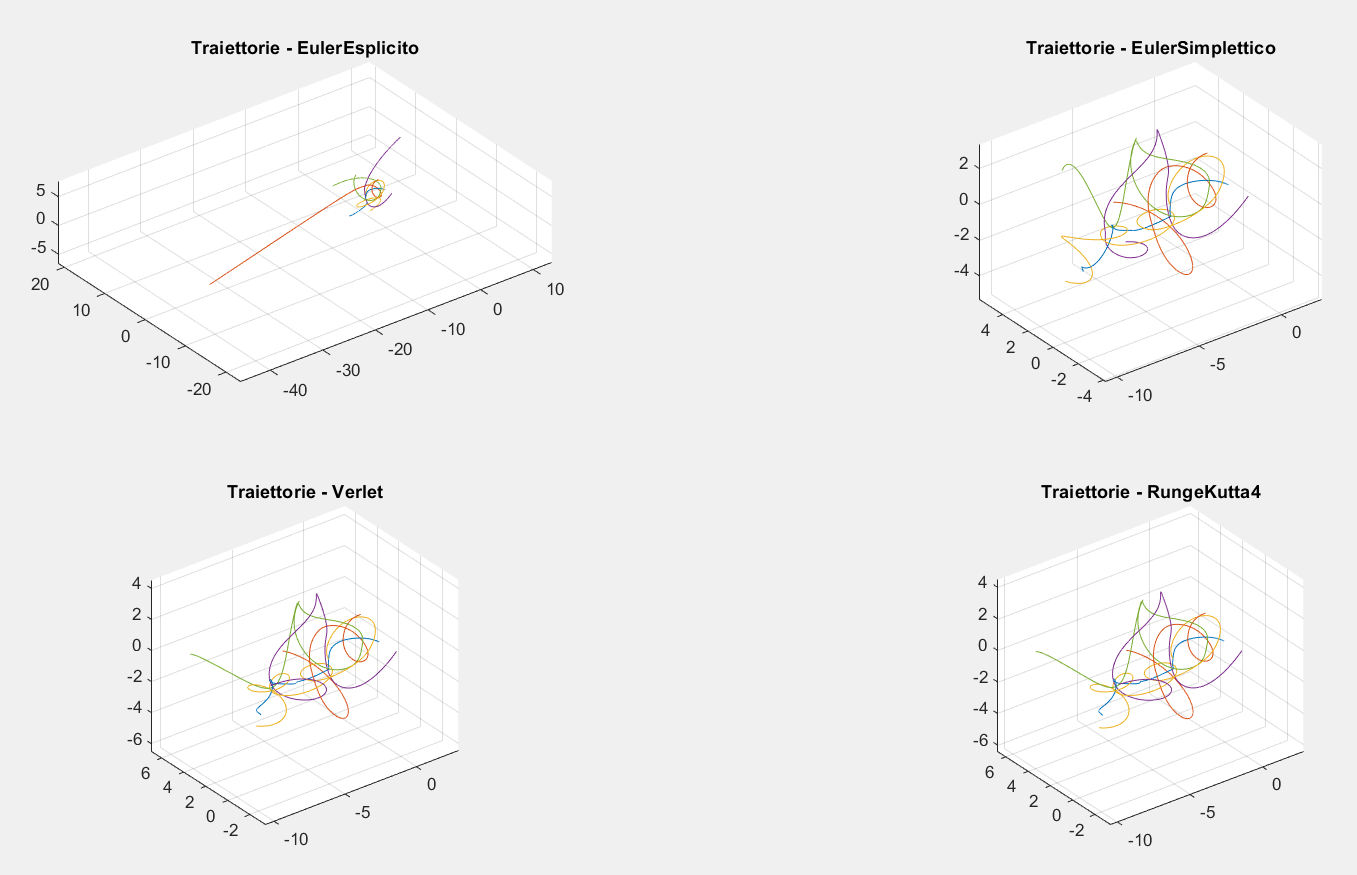
\includegraphics[width=1\textwidth]{trajectories_comparison.png}
    \caption{Confronto delle traiettorie dei corpi tra i vari metodi.}
\end{figure}

I metodi simplettici (Eulero simplettico e Verlet) mostrano una buona conservazione dell'energia nel lungo periodo, con il secondo sempre più preciso del primo. 
\\ Nonostante RK4 abbia un'alta precisione locale, esso pu\`o introdurre deriva energetica. (Fig. 3)\\ Infine, il metodo di Eulero esplicito risulta spesso instabile con errori crescenti nel tempo.

\begin{figure}[H]
    \centering
    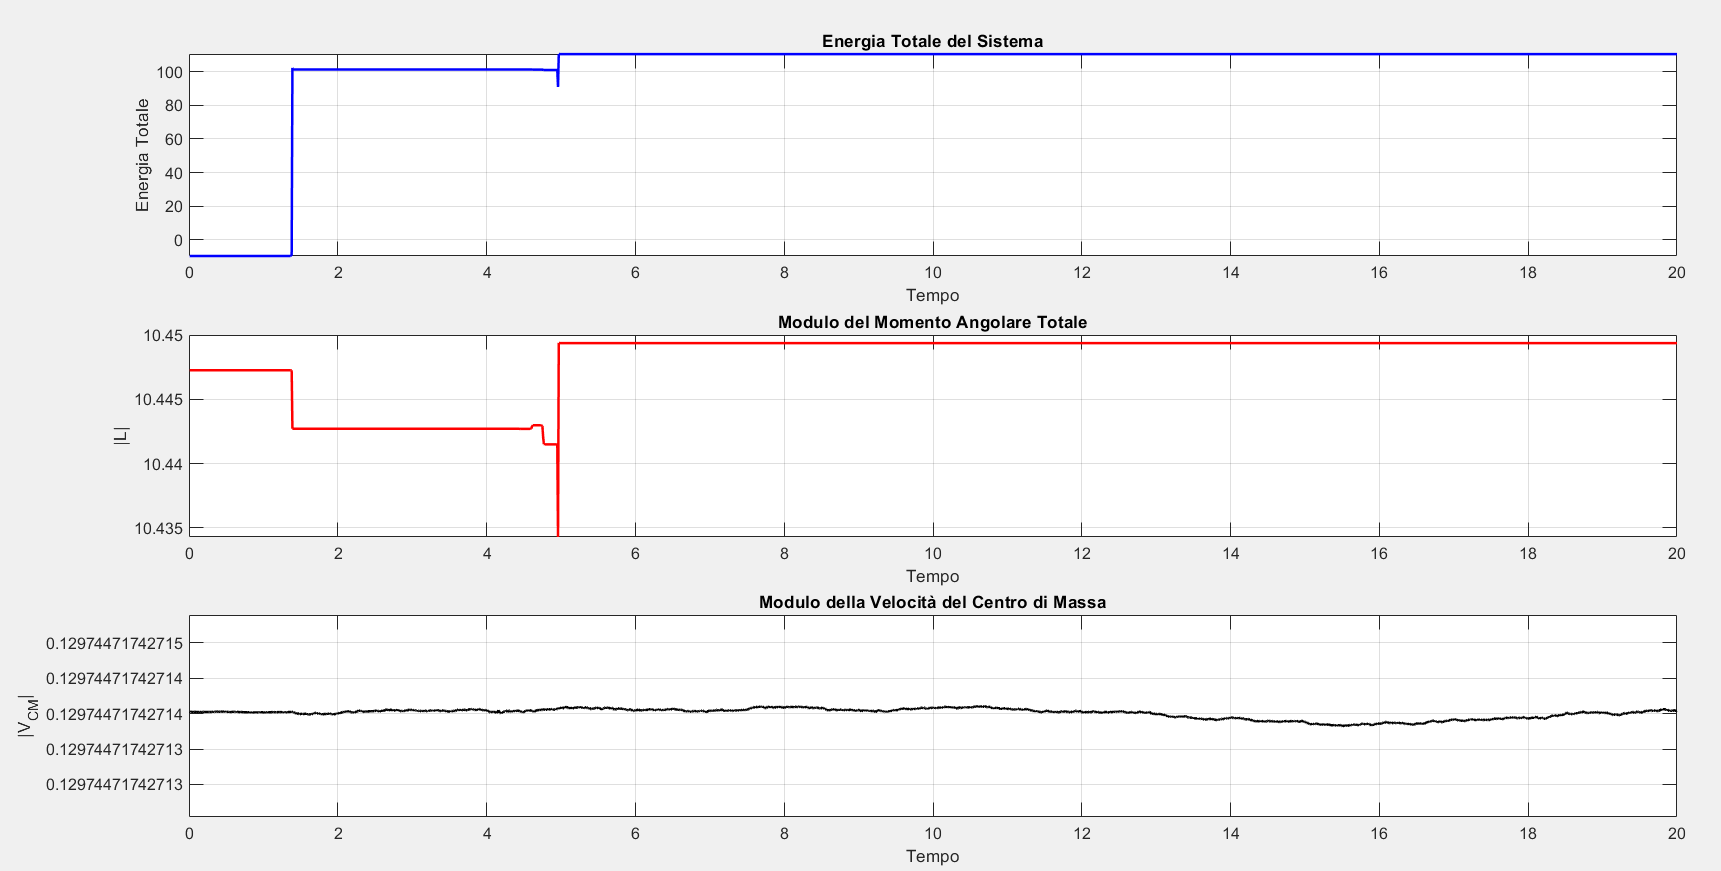
\includegraphics[width=1\textwidth]{rk4_conservations.png}
    \caption{Grafico delle conservazioni con RK4 con n=10 e dt=0.01}
\end{figure}

\section{Comportamento caotico e sensibilità alle condizioni iniziali}

Il problema degli \(n\)-corpi newtoniano è noto per il suo comportamento caotico, specialmente in assenza di una massa dominante e quando tutte le masse sono comparabili. In questa sezione analizziamo la sensibilità del sistema alle condizioni iniziali, utilizzando una configurazione in cui tutte le masse sono unitarie e si distribuiscono inizialmente attorno a un centro comune.

Per mettere in evidenza il carattere caotico del sistema, abbiamo eseguito due simulazioni parallele: la prima con le condizioni iniziali standard, la seconda con una lieve perturbazione sulla posizione di un singolo corpo. In particolare, al vettore posizione del secondo corpo è stato sommato un piccolo vettore casuale \(\varepsilon \, \mathbf{u}\), dove \(\varepsilon = 10^{-4}\) e \(\mathbf{u}\) è un vettore unitario casuale.

Le due simulazioni sono state integrate usando lo stesso metodo numerico (in questo caso, il metodo di Verlet), e ad ogni passo temporale abbiamo misurato la **divergenza** tra le due evoluzioni come la somma delle distanze euclidee tra le posizioni corrispondenti dei corpi:

\[
\Delta(t) = \sum_{i=1}^{n} \left\| \mathbf{r}_i(t) - \mathbf{r}_i'(t) \right\|,
\]

dove \(\mathbf{r}_i(t)\) è la posizione del corpo \(i\) nella simulazione originale e \(\mathbf{r}_i'(t)\) quella nella simulazione perturbata. L'andamento temporale di \(\Delta(t)\) è riportato nel grafico seguente, e mostra un comportamento tipicamente esponenziale, segno della forte dipendenza del sistema dalle condizioni iniziali.

\begin{figure}[h!]
    \centering
    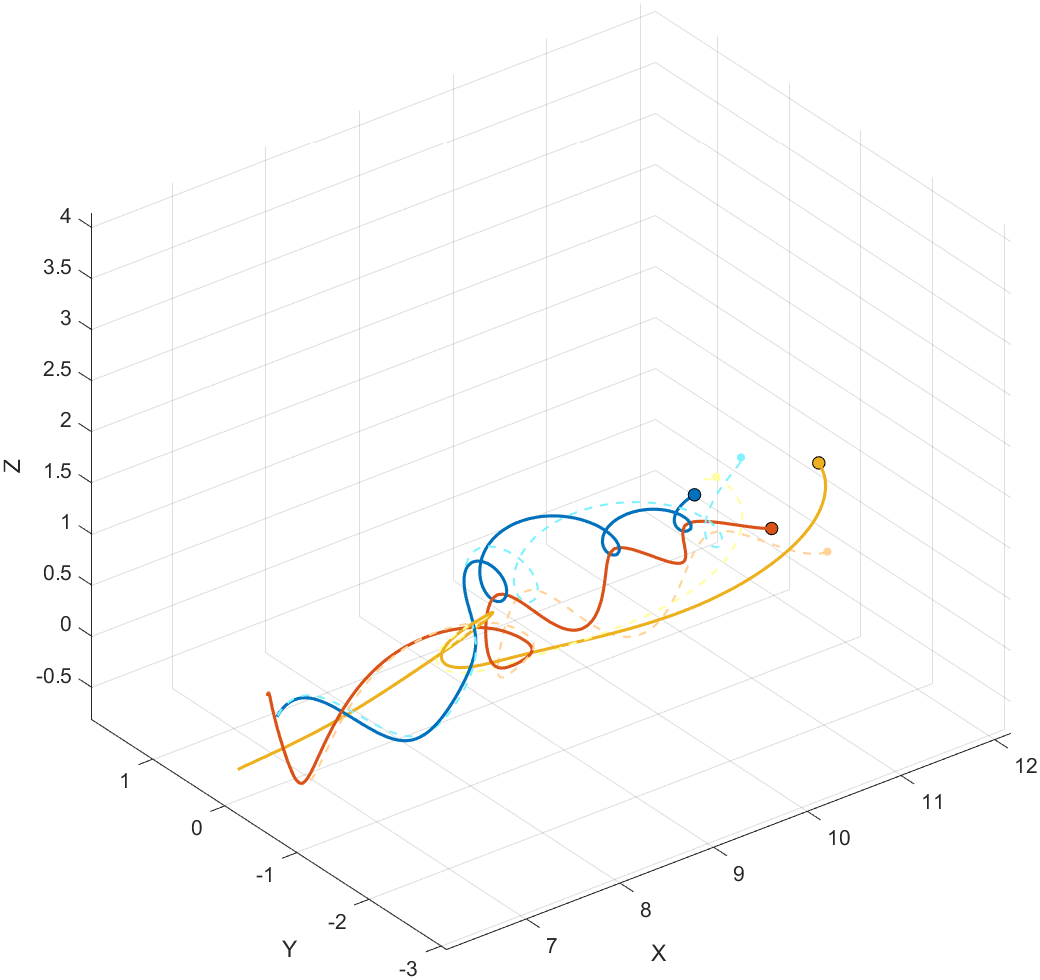
\includegraphics[width=0.75\textwidth]{cahotic_traj.png}
    \caption{Tracciamento delle traiettorie dei corpi per due simulazioni: una con condizioni iniziali originali e una leggermente perturbata. Le traiettorie della simulazione perturbata sono desaturate.}
    \label{fig:traiettorie}
\end{figure}

\begin{figure}[h!]
    \centering
    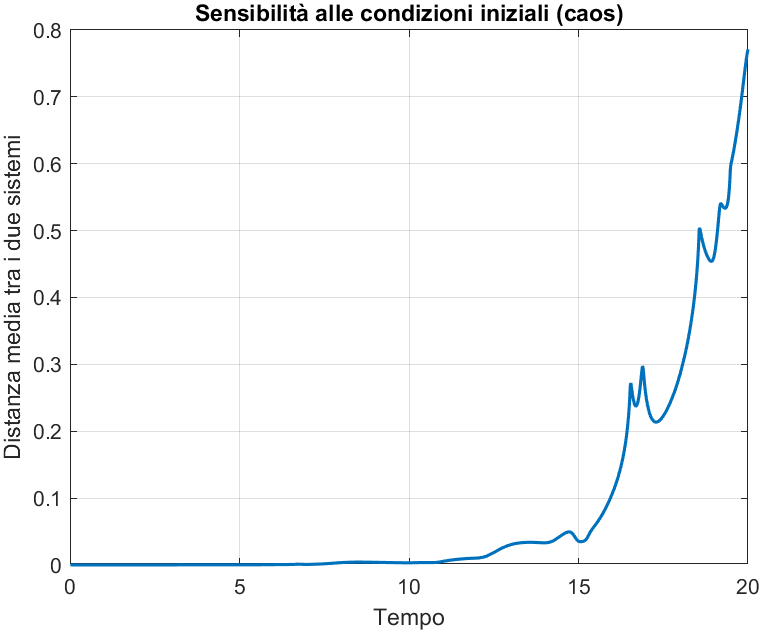
\includegraphics[width=0.65\textwidth]{cahotic_div.png}
    \caption{Andamento della divergenza \(\Delta(t)\) tra le due simulazioni nel tempo. Il comportamento caotico si manifesta nella crescita esponenziale della distanza tra le due evoluzioni.}
    \label{fig:divergenza}
\end{figure}

Questi risultati confermano che, nonostante il sistema sia completamente deterministico, piccole incertezze nelle condizioni iniziali rendono impraticabile una previsione accurata a lungo termine. Questo comportamento è una manifestazione del caos deterministico tipico dei sistemi non lineari con più di due corpi in interazione gravitazionale.


\section{Conclusioni}
Il confronto ha evidenziato come i metodi simplettici siano particolarmente adatti per sistemi hamiltoniani a lungo termine. Verlet, in particolare, combina buona stabilit\`a numerica e conservazione dell'energia. RK4 resta utile per accuratezza immediata ma va usato con cautela. L'analisi lagrangiana e hamiltoniana fornisce il quadro teorico per interpretare i comportamenti osservati nei metodi numerici.

\end{document}

